%%%%%%%%%%%%%%%%%%%%%%%%%%%%%%%%%%%%%%%%%
% Stylish Article
% LaTeX Template
% Version 2.2 (2020-10-22)
%
% This template has been downloaded from:
% http://www.LaTeXTemplates.com
%
% Original author:
% Mathias Legrand (legrand.mathias@gmail.com) 
% With extensive modifications by:
% Vel (vel@latextemplates.com)
%
% License:
% CC BY-NC-SA 3.0 (http://creativecommons.org/licenses/by-nc-sa/3.0/)
%
%%%%%%%%%%%%%%%%%%%%%%%%%%%%%%%%%%%%%%%%%

%----------------------------------------------------------------------------------------
%	PACKAGES AND OTHER DOCUMENT CONFIGURATIONS
%----------------------------------------------------------------------------------------

\documentclass[fleqn,10pt]{SelfArx} % Document font size and equations flushed left
\usepackage[english]{babel} % Specify a different language here - english by default

\usepackage{lipsum} % Required to insert dummy text. To be removed otherwise
\usepackage{tikz}
\usepackage{tikzit}
\usepackage{adjustbox}
\usepackage{graphicx}
\usepackage{xcolor}
\usepackage{listings}

\usepackage{xparse}

\NewDocumentCommand{\codeword}{v}{%
\texttt{\textcolor{blue}{#1}}%
}
\graphicspath{ {./figures/} }

%----------------------------------------------------------------------------------------
%	COLUMNS
%----------------------------------------------------------------------------------------

\setlength{\columnsep}{0.55cm} % Distance between the two columns of text
\setlength{\fboxrule}{0.75pt} % Width of the border around the abstract

%----------------------------------------------------------------------------------------
%	COLORS
%----------------------------------------------------------------------------------------

\definecolor{color1}{RGB}{0,0,90} % Color of the article title and sections
\definecolor{color2}{RGB}{0,20,20} % Color of the boxes behind the abstract and headings

%----------------------------------------------------------------------------------------
%	HYPERLINKS
%----------------------------------------------------------------------------------------

\usepackage{hyperref} % Required for hyperlinks

\hypersetup{
	hidelinks,
	colorlinks,
	breaklinks=true,
	urlcolor=color2,
	citecolor=color1,
	linkcolor=color1,
	bookmarksopen=false,
	pdftitle={Title},
	pdfauthor={Author},
}

%----------------------------------------------------------------------------------------
%	ARTICLE INFORMATION
%----------------------------------------------------------------------------------------

% \JournalInfo{Journal, Vol. XXI, No. 1, 1-5, 2013} % Journal information
% \Archive{Additional note} % Additional notes (e.g. copyright, DOI, review/research article)

\PaperTitle{BudgetLambda - Quick Serverless Pipelines} % Article title

\Authors{Donglin Xu, Yiheng Niu, Qiu Chen} % Authors
\affiliation{\textsuperscript{1}\textit{Department of Biology, University of Examples, London, United Kingdom}} % Author affiliation
\affiliation{\textsuperscript{2}\textit{Department of Chemistry, University of Examples, London, United Kingdom}} % Author affiliation
\affiliation{*\textbf{Corresponding author}: john@smith.com} % Corresponding author

\Keywords{Keyword1 --- Keyword2 --- Keyword3} % Keywords - if you don't want any simply remove all the text between the curly brackets
\newcommand{\keywordname}{Keywords} % Defines the keywords heading name
\newcommand{\CSh}{C\nolinebreak\hspace{-.05em}\raisebox{.6ex}{\scriptsize\bf \#}}

%----------------------------------------------------------------------------------------
%	ABSTRACT
%----------------------------------------------------------------------------------------

% \Abstract{Lorem ipsum dolor sit amet, consectetuer adipiscing elit. Ut purus elit, vestibulum ut, placerat ac, adipiscing vitae, felis. Curabitur dictum gravida mauris. Nam arcu libero, nonummy eget, consectetuer id, vulputate a, magna. Donec vehicula augue eu neque. Pellentesque habitant morbi tristique senectus et netus et malesuada fames ac turpis egestas. Mauris ut leo. Cras viverra metus rhoncus sem. Nulla et lectus vestibulum urna fringilla ultrices. Phasellus eu tellus sit amet tortor gravida placerat. Integer sapien est, iaculis in, pretium quis, viverra ac, nunc. Praesent eget sem vel leo ultrices bibendum. Aenean faucibus. Morbi dolor nulla, malesuada eu, pulvinar at, mollis ac, nulla. Curabitur auctor semper nulla. Donec varius orci eget risus. Duis nibh mi, congue eu, accumsan eleifend, sagittis quis, diam. Duis eget orci sit amet orci dignissim rutrum.}

%----------------------------------------------------------------------------------------

\begin{document}
\nocite{*}

\maketitle % Output the title and abstract box

\tableofcontents % Output the contents section

\thispagestyle{empty} % Removes page numbering from the first page

%----------------------------------------------------------------------------------------
%	ARTICLE CONTENTS
%----------------------------------------------------------------------------------------

\section*{Introduction} % The \section*{} command stops section numbering

\addcontentsline{toc}{section}{Introduction} % Adds this section to the table of contents

\indent \emph{BudgetLambda} is a user-friendly and versatile tool for constructing and deploying data processing pipelines that supports a variety of programming languages. It is built on top of a Kubernetes cluster and draws inspiration from recent concepts in serverless computing and distributed systems.

At the heart of BudgetLambda is an automated image engine that arranges user-supplied short code snippets (lambdas) into a cohesive pipeline. These components are linked together to facilitate rapid prototyping across diverse programming languages. The platform allows for the independent scaling of each component according to workload demands, ensuring efficient resource utilization and optimal performance.

The primary objective of BudgetLambda is to offer a collaborative environment that enables small groups with disparate technical backgrounds to collaborate effectively. By facilitating quick prototyping of key services, the tool provides an expedited pathway to transitioning into a custom-built end-to-end solution.

%------------------------------------------------

\section{Architecture}

\indent \emph{BudgetLambda} is a software solution that leverages multiple open-source tools and custom libraries to enable its infrastructure. At the core of the project lies \par \noindent
\texttt{BudgetLambda.CoreLib}, which provides abstractions for individual components and enables communication between infrastructural software packages. A long-running web UI, \texttt{BudgetLambda.Server}, sits on top of the core library and serves as the primary interface for users.

The entire project, including user-defined software components, is designed to run on a Kubernetes cluster, ensuring efficient deployment and operations. Data storage and persistence are facilitated by a PostgreSQL database, while the ORM layer provides abstractions that enable the plugging in of other databases. User-defined functions are deployed using \texttt{OpenFaas}, and container building and storage are facilitated by \texttt{Docker}.

The integration of open-source tools and custom libraries enables \emph{BudgetLambda} to offer a robust and scalable solution. The use of Kubernetes as the deployment environment further enhances the platform's operational efficiency, while the PostgreSQL database provides reliable data storage and persistence. The deployment of user-defined functions on \texttt{OpenFaas} and containerization using Docker enables \emph{BudgetLambda} to offer an efficient and user-friendly interface for constructing and deploying data processing pipelines.

In summary, BudgetLambda offers a sophisticated and comprehensive infrastructure that is built upon a variety of open-source tools and custom libraries. Its deployment on a Kubernetes cluster, use of \texttt{PostgreSQL} for data storage and persistence, and deployment of user-defined functions on \texttt{OpenFaas} using Docker containerization, enable BudgetLambda to provide an accessible platform for building and deploying data processing pipelines.

\subsection{Core Components}

\subsubsection{BudgetLambda.CoreLib}

The \emph{BudgetLambda.CoreLib} library serves as a foundational component of the system and provides abstractions that encapsulate the core functionality. Its primary feature is the ability to construct individual \emph{Pipeline Packages}, which contain component information, data flow, and data schema between each component. These packages can be scheduled onto the Kubernetes cluster through a \emph{Scheduler} that configures the pipeline and populates runtime execution information before performing the necessary packaging and deployment.

To facilitate the deployment of components, the library defines an overall abstraction class called \emph{ComponentBase}. This class serves as a base for implementations and provides the common traits required before a component can be scheduled. Within each individual implementation of \emph{ComponentBase}, additional information such as health checking and log aggregation is performed. This functionality enables users to observe the deployment without resorting to external toolchains, thereby streamlining the development and deployment process.

Overall, the \emph{BudgetLambda.CoreLib} library serves as a vital component of the system, providing essential abstractions and functionality for constructing and deploying data processing pipelines. Its ability to encapsulate core functionality and deploy components efficiently on a Kubernetes cluster enables users to focus on pipeline design and development, while the library handles the underlying infrastructure.

\subsubsection{BudgetLambda.Server}

The \emph{BudgetLambda.Server} sub-project is a long-running web service designed to provide users with an intuitive user interface for building pipelines and components. It incorporates basic user-based authentication for multi-tenant use scenarios. The front-end is developed entirely in .NET, adhering to modern front-end standards with a server-rendered SPA structure.

The \emph{BudgetLambda.CoreLib} is embedded directly in the server, with individual functionality directly injected into pages, thereby allowing for swift interaction with the underlying infrastructure. This integration streamlines the development and deployment process, enabling users to focus on pipeline design and component development without having to worry about the underlying infrastructure. Overall, the \emph{BudgetLambda.Server} sub-project plays a crucial role in providing a user-friendly interface for pipeline design and deployment, thereby facilitating efficient and effective data processing.

\subsubsection{BudgetLambda.BakedComponents}

The initial release of \emph{BudgetLambda} comes with a set of reference components that showcase the core concepts of the project through several common use scenarios. Due to time constraints, the number of baked-in components is limited and they only cover a specific range of programming languages and use cases. These components serve as reference points for future development, rather than an exhaustive set.

\emph{BudgetLambda.HttpSource} implements a data source for the pipeline, exposes an HTTP endpoint for data input.

\emph{BudgetLambda.CSharpLambdaMap}, \\ \emph{BudgetLambda.JavascriptLambdaMap} and \\ \emph{BudgetLambda.PythonLambdaMap} implements a serverless function snippet template that takes in a user-defined function, passes upstream input data to be handled by the user function, then sending processed data towards downstream components.

\emph{BudgetLambda.StdOutSink} implements a simple sink that takes upstream data and prints them into stdout.

\emph{BudgetLambda.EmailSink} implements a sink that takes upstream data and sends the results using email to an address specified by upstream.

\subsection{Infrastructural Components}

\subsubsection{Kubernetes}

This software project is designed to operate on a Kubernetes cluster, which provides a highly scalable and fault-tolerant infrastructure for real-time traffic demands. The main user interaction point, \emph{BudgetLambda.Server}, is containerized without stateful dependencies, allowing it to efficiently scale up and down as needed. The scheduler automatically packages and deploys user-defined components into container images, which are then scheduled onto the cluster. With the use of Kubernetes, individual stages in the data processing pipeline can be scaled independently, increasing the overall efficiency of the infrastructure. In the event of catastrophic failures in compute nodes, the system is designed to maintain its fault-tolerant characteristics, ensuring a reliable and stable user experience.

\subsubsection{Docker Engine}

The project leverages the widely adopted Docker image format to package user-defined components and packages. Once packaged, these images are stored in a private image registry, from where they can be scheduled to run on a Kubernetes cluster. It is noteworthy that Docker engine is only employed for image building and storage, while containerd serves as the preferred container runtime in this project.

\subsubsection{RabbitMQ}

The project utilizes RabbitMQ as a messaging broker for inter-component communication, specifically for message queuing between upstream and downstream components. The system creates a "Master Exchange" for each package, with individual components configured with unique routing keys based on their position in the pipeline. This approach aims to ensure optimal distribution and handling of messages between components, particularly in high scalability scenarios.

\subsubsection{PostgreSQL}

Data, package, and component definitions as well as serverless code snippets submitted by users are stored in a distinct PostgreSQL database server located outside of the Kubernetes cluster. To facilitate database access, \emph{BudgetLambda.CoreLib} utilizes an object-relational mapping (ORM) framework, obviating the need for raw SQL queries. PostgreSQL was chosen for its performance and versatility. However, it is possible to incorporate other databases through the abstraction layer, which is vendor-neutral.

\subsection{Component Relations}

The core access point for the system is the \\ \emph{BudgetLambda.Server} which is embedded with \\ \emph{BudgetLambda.Corelib} that exposes the central abstractions to users. The user can define pipeline packages and components via the web interface and store them in a PostgreSQL database. Subsequently, the user-defined components are combined with corresponding programming language templates, and the resulting code is pushed to a remote docker server for image building. The final container images are then pushed to a remote docker registry, and made available for deployment. The Scheduler processes these images according to the configuration of the components in the pipeline, ensuring that data flows correctly between them via the message queue. Once the Scheduler has completed its configuration, it schedules these components on the Kubernetes cluster for execution.

\begin{figure}
	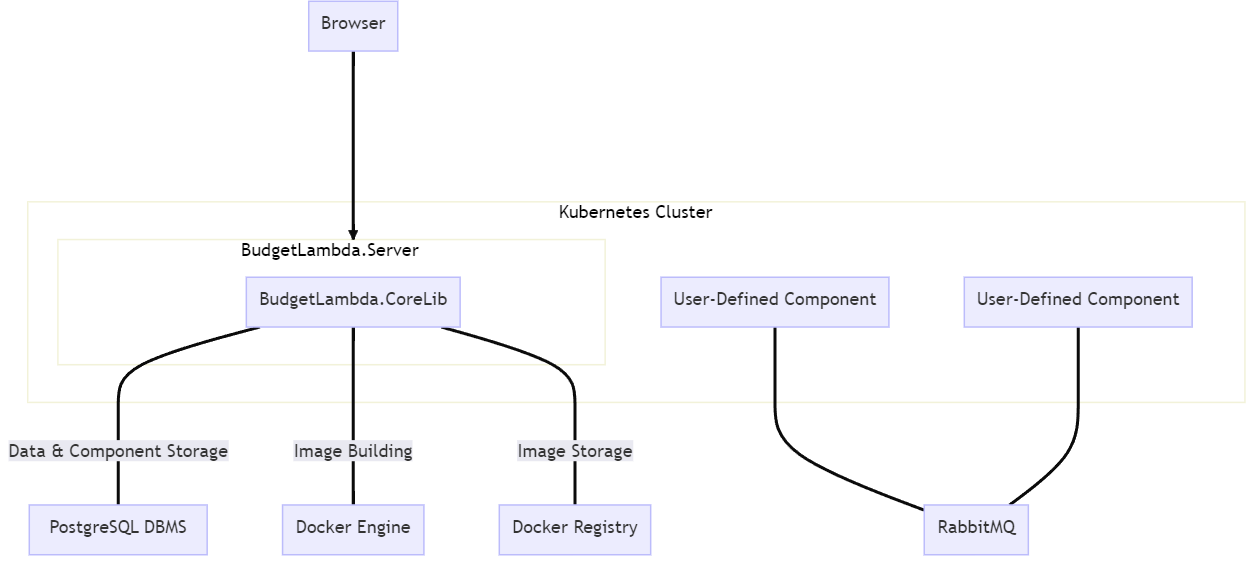
\includegraphics[width=\columnwidth]{fig1}
\end{figure}


%------------------------------------------------

\section{Operations Overview}

As \emph{BudgetLambda} relies on multiple underlying infrastructural components, the preparation and configuration of these components can pose challenges. This chapter provides detailed guidance on the deployment and configuration of various dependencies, including \emph{BudgetLambda} itself, to ensure proper functioning of the system. The focus is on accurate configuration and optimal setup of the individual components, considering their interdependencies and interactions within the overall system architecture.

\subsection{Infrastructure Preparation}

\subsubsection{Kubernetes}

To achieve optimal performance and fault-tolerance in the system, a minimum set of recommendations for each compute node in the cluster is summarized in the table below.

\begin{table}[hbt]
	\caption{Hardware Recommendation}
	\centering
	\begin{tabular}{llr}
		\toprule
		Processor Cores & RAM & Storage Type \\
		\midrule
		4 & 8 GiB & SSD \\
		\bottomrule
	\end{tabular}
\end{table}

It is recommended to have at least 3 compute nodes in the cluster. \\

\emph{BudgetLambda} leverages \emph{OpenFaaS} for seamless deployment of user-defined serverless functions. As part of the system setup, \emph{OpenFaaS} should be installed in the cluster and configured to expose its HTTP endpoint either through a load balancer or ingress. This ensures smooth integration of serverless functions into the overall system architecture, enabling efficient handling of user-defined code snippets within the \emph{BudgetLambda} environment.


\subsubsection{Database}

The system is designed to utilize an external PostgreSQL database server for storing user information, package and component definitions as the default configuration. It is recommended to set up the database outside of the cluster in a dedicated server. However, \emph{BudgetLambda.CoreLib} provides the flexibility to use other database systems through modifications in the ORM layer, as outlined in the development guide. Data storage and querying in the system are achieved exclusively through the ORM, eliminating the need for raw SQL queries and maintaining vendor-neutral access in case of a switch to a different database system. \emph{BudgetLambda} adopts the Table-per-Hierarchy style of schema modeling, with a discriminator column indicating the exact type of data. To ensure optimal performance for database access, a sample configuration for PostgreSQL is provided to guide the system configuration process. This approach ensures efficient and reliable database operations within the \emph{BudgetLambda} system, enabling seamless data storage and retrieval for various use cases.

\begin{verbatim}
# DB Version: 15
# OS Type: linux
# DB Type: web
# Total Memory (RAM): 8 GB
# CPUs num: 4
# Data Storage: ssd

max_connections = 200
shared_buffers = 2GB
effective_cache_size = 6GB
maintenance_work_mem = 512MB
checkpoint_completion_target = 0.9
wal_buffers = 16MB
default_statistics_target = 100
random_page_cost = 1.1
effective_io_concurrency = 200
work_mem = 5242kB
min_wal_size = 1GB
max_wal_size = 4GB
max_worker_processes = 4
max_parallel_workers_per_gather = 2
max_parallel_workers = 4
max_parallel_maintenance_workers = 2
\end{verbatim}

\subsubsection{RabbitMQ}

Within the \emph{BudgetLambda} system, RabbitMQ is employed as the internal message broker for communication between components. Each package in the system is associated with a master exchange that efficiently handles and routes all messages produced by the components. The configuration of the message broker is automatically managed by the project based on user-defined metadata, eliminating the need for manual operations. To ensure a high degree of fault-tolerance, it is recommended to have a minimum of three nodes in the RabbitMQ cluster. This approach guarantees reliable and efficient message communication among components in the \emph{BudgetLambda} system, facilitating seamless coordination and interaction between different modules.

\subsection{Deployment Considerations}

\subsubsection{Server Deployment}
The architecture of \emph{BudgetLambda} is designed to be stateless, with all the data required by the system stored external to the container. User information and package definitions are stored in the dedicated database, while server configuration is loaded via its configuration interface. It is recommended to define the configuration as a ConfigMap resource in the Kubernetes cluster, which can be mounted into the container for easy access. Alternatively, sensitive data can also be securely passed to the container through environment variables. This approach ensures that the system remains stateless, allowing for efficient scaling, high availability, and ease of management in a containerized environment.

\subsubsection{Monitoring}
Both the server and user-defined components in \\ \emph{BudgetLambda} generate logs that are emitted to the console during system operation. To ensure effective monitoring of the system in real-time, we recommend deploying a log-aggregation tool that can collect and analyze these logs. Furthermore, \emph{BudgetLambda.Server} provides a dedicated interface for displaying component logs to the user, which is achieved through the embedding of individual Grafana dashboards at the management page of each component. This feature enhances system visibility and facilitates effective troubleshooting and performance analysis of the components.

\section{Development Guide}

\subsection{Component Overview}

In the development framework of \emph{BudgetLambda}, components are designed to inherit from the \codeword{ComponentBase} class and override a set of virtual and abstract methods. This enables seamless integration of components with the packaging and scheduling engine, allowing users to construct individual components within a pipeline. Generally, there are two categories of components: \codeword{Source}, \codeword{Sink}, and \codeword{Lambda Map}, each serving a specific role in the pipeline. A pipeline can have only one \codeword{Source} component, which acts as the entry point for data into the package. By default, \emph{BudgetLambda} provides an \codeword{HttpSink} component that exposes an external HTTP endpoint for accepting JSON-formatted data. \codeword{Lambda Map} components represent user-defined code snippets, typically implemented as single functions that receive input from upstream components and produce output for downstream components. The initial release of \emph{BudgetLambda} supports \CSh, Python, and JavaScript as available languages for implementing \codeword{ComponentBase} subclasses, although other languages can also be integrated. \codeword{Sink} components, located at the end of the pipeline, perform necessary operations to consume the transformed data. In the initial release, there are two sink components available, namely \codeword{StdoutSink} and \codeword{EmailSink}. As the names suggest, the former prints the data in the console for debugging purposes, while the latter sends an email to a designated address.

\subsubsection{Templated Components}

The \codeword{Lambda Map} components in \emph{BudgetLambda} are designed to be "Templated," which means that they are composed of a pre-built execution environment image (referred to as a template) and a user-defined code snippet that is attached to the template. The implementation of these components involves a two-stage image building process, where the first stage prepares the template and the second stage combines the user code with the template. Detailed information about the development process for these components will be provided in the upcoming chapter.

\subsubsection{Non-Template Components}

The \codeword{Source} and \codeword{Sink} components in \emph{BudgetLambda} are typically designed to obtain user-provided configuration directly through their environment, without the need for re-building. These components can be fully pre-built and stored in the image registry. The corresponding implementations of their \codeword{ComponentBase} subclasses should directly return from the image building methods, allowing the scheduling engine to handle deployment operations accurately.


\begin{table}[hbt]
	\caption{Initial Release Components}
	\centering
	\begin{tabular}{llll}
		\toprule
		Name & Type & Category & Language \\
		\midrule
		HttpSource & Source & Pre-Built & N/A \\
		CSharpLambdaMap & Lambda Map & Template & \CSh \\
		JavaScriptLambdaMap & Lambda Map & Template & JavaScript \\
		PythonLambdaMap & Lambda Map & Template & Python \\
		StdoutSink & Sink & Pre-Built & N/A \\
		EmailSink & Sink & Pre-Built & N/A \\
		\bottomrule
	\end{tabular}
\end{table}


\end{document}